\renewcommand{\nrandom}{\num{700}}
\renewcommand{\napplication}{\num{212}}
\newcommand{\ntoilet}{\num{77}}
\newcommand{\nmaxcount}{\num{26}}
\newcommand{\nsandcastle}{\num{25}}
\newcommand{\nconformant}{\num{24}}
\newcommand{\nmpec}{\num{60}}

\section{Evaluation}
\label{sect:erssat-evaluation}

We evaluated the proposed~\cref{alg:erssat} against
the state-of-the-art DPLL-based SSAT solver \dcssat~\cite{Majercik2005}
over both random $k$-CNF and application formulas.
The proposed algorithm is implemented in the \texttt{C++} language inside the \abc~\cite{ABC} environment.
The SAT solver \minisat-2.2~\cite{Een2003Solver} is used to answer satisfiability queries.
For weighted model counting,
we tried \cachet~\cite{Sang2004,Sang2005ModelCounting},
but the overall performance was not satisfactory.
Instead, we resorted to a well-developed BDD package \cudd~\cite{CUDD}.
Weight computation of a formula is fulfilled via a classic approach~\cite{Darwiche2002KnowledgeCompilation} that traverses the BDD of a formula and computes the satisfying probabilities of the BDD nodes.
Our prototyping implementation\footnote{Available at: \url{\ssatabcurl}} is named \erssat.
A bare version of \erssat without the enhancement techniques is called \erssatb in the experiments.
We used \ssatABCRevision in the experiments.

\subsection{Benchmark set}
The SSAT instances in the evaluation are hosted
in a publicly available database\footnote{Available at: \url{\ssatbenchmarkurl}}.
We used \ssatBenchRevision in the experiments.

\subsubsection{Random $k$-CNF formulas}
We generated random $k$-CNF formulas by \cnfgen~\cite{Lauria2017CNFgen}.
A collection of~\nrandom~formulas were generated with $k$,
i.e., the number of literals in a clause,
taking values from $\{3,4,5,6,7,8,9\}$,
the number of variables taking values from $\{10,20,30,40,50\}$,
and clause-to-variable ratio taking values from $\{k-1,k,k+1,k+2\}$.
Five formulas were sampled for each parameter combination.
To convert the propositional formulas into E-MAJSAT formulas,
the first half of the variables are existentially quantified,
and the rest are randomly quantified with probability $0.37$.

\subsubsection{Application formulas}
\begin{table}[ht]
    \centering
    \caption{The families of the application formulas}
    \label{tbl:exist-random-ssat-families}
    \begin{tabular}{c|c|c}
        Family               & Description                                            & Number       \\
        \hline
        \textit{Toilet-A}    & Adapted from exist-forall QBFs~\cite{Narizzano2006}    & \ntoilet     \\
        \textit{Conformant}  & Adapted from exist-forall QBFs~\cite{Narizzano2006}    & \nconformant \\
        \textit{Sand-Castle} & A probabilistic planning problem~\cite{Majercik1998}   & \nsandcastle \\
        \textit{Max-Count}   & Adapted from maximum model counting~\cite{Fremont2017} & \nmaxcount   \\
        \textit{MPEC}        & Maximum probabilistic equivalence checking             & \nmpec       \\
    \end{tabular}
\end{table}

We collected five families of application formulas for evaluation.
Their descriptions and the numbers of the instances in each family are summarized in~\cref{tbl:exist-random-ssat-families}.
The first two families,
\textit{Toilet-A} and \textit{Conformant},
were adapted from exist-forall-exist QBFs~\cite{Narizzano2006}.
We converted the QBFs into exist-random-exist quantified SSAT formulas
by replacing their universal quantifiers with randomized ones with probabilities $0.5$.
The third family \textit{Sand-Castle} is a probabilistic conformant planning domain.
The problem can be encoded as E-MAJSAT formulas~\cite{Majercik1998}.
The family \textit{Max-Count} models the problems of maximum satisfiability, quantitative information flow, and program synthesis with maximum model counting~\cite{Fremont2017}.
We represented the maximum model counting instances as E-MAJSAT formulas.
The last family \textit{MPEC} consists of formulas that analyze the maximum probability of a probabilistic circuit to produce erroneous outputs,
as discussed in~\cref{chap:prob-design-eval}.

\subsection{Experimental setup}
Our experiments were performed on a machine with~\machineSpec.
The operating system was~\osInfo.
The programs were compiled with~\compiler.
Each SSAT-solving task was limited to a CPU core,
a CPU time of~\timelimit,
and a memory usage of~\memlimit.
To achieve reliable benchmarking,
we used a benchmarking framework \benchexec\footnote{Available at: \url{\benchexecurl}}~\cite{Benchmarking-STTT}.

\subsection{Results}

\subsubsection{Random $k$-CNF formulas}

\begin{figure*}[hp]
    \centering
    \subfloat[CPU time]{
        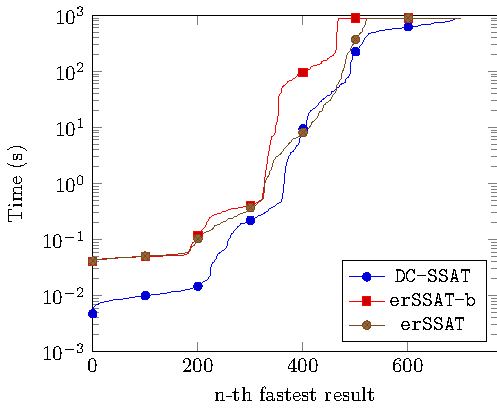
\includegraphics{exist-random-ssat/evaluation/plots/quantile-cputime-Random.pdf}
        \label{fig:erssat-quantile-cputime-random}
    }\\
    \subfloat[Memory usage]{
        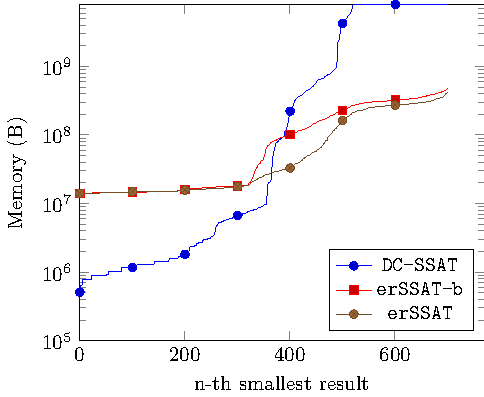
\includegraphics{exist-random-ssat/evaluation/plots/quantile-memory-Random.pdf}
        \label{fig:erssat-quantile-memory-random}
    }
    \caption{Quantile plots of random $k$-CNF formulas}
    \label{fig:erssat-quantile-random}
\end{figure*}

\Cref{fig:erssat-quantile-random} shows the quantile plots regarding CPU time and memory usage
of the SSAT instances derived from the random $k$-CNF formulas.
A data point $(x,y)$ in a quantile plot indicates that
there are $x$ formulas processed by the respective algorithm within a resource constraint of $y$.
In~\cref{fig:erssat-quantile-cputime-random},
we observe that \erssat solved a similar amount of formulas as \dcssat did.
Moreover, the enhancement techniques improve the performance of \erssat a lot,
as can be seen from the huge difference between \erssat and \erssatb.
On the other hand,
\cref{fig:erssat-quantile-memory-random} shows that \dcssat used much more memory than \erssat.
This can be attributed to the subformula caching of \dcssat.
Instead, \erssat only builds BDDs for cofactored formulas, which confined its memory footprint.

\subsubsection{Application formulas}

% Commands for application formulas of ER-SSAT
\newcommand{\dcssatToiletA}{\num{44}}
\newcommand{\dcssatconformant}{\num{1}}
\newcommand{\dcssatcastle}{\num{21}}
\newcommand{\dcssatMaxCount}{\num{2}}
\newcommand{\dcssatMPEC}{\num{3}}
\newcommand{\erssatbToiletA}{\num{45}}
\newcommand{\erssatbconformant}{\num{1}}
\newcommand{\erssatbcastle}{\num{14}}
\newcommand{\erssatbMaxCount}{\num{1}}
\newcommand{\erssatbMPEC}{\num{1}}
\newcommand{\erssatToiletA}{\num{38}}
\newcommand{\erssatconformant}{\num{2}}
\newcommand{\erssatcastle}{\num{13}}
\newcommand{\erssatMaxCount}{\num{3}}
\newcommand{\erssatMPEC}{\num{2}}

\begin{table}[t]
    \centering
    \caption{Summary of the results for~\napplication~application formulas}
    \label{tbl:exist-random-ssat-application}
    \begin{tabular}{l|ccc}
        \toprule
        Algorithm                   & {\dcssat}                                                     & {\erssat} & {\erssatb} \\
        \midrule
        Solved formulas             & \num{\DcssatErDefaultApplicationMissingCount}
                                    & \num{\ErssatDefaultBddApplicationMissingCount}
                                    & \num{\ErssatBareBddApplicationMissingCount}                                            \\
        \qquad \textit{Toilet-A}    & \num{\dcssatToiletA}
                                    & \num{\erssatToiletA}
                                    & \num{\erssatbToiletA}                                                                  \\
        \qquad \textit{Conformant}  & \num{\dcssatconformant}
                                    & \num{\erssatconformant}
                                    & \num{\erssatbconformant}                                                               \\
        \qquad \textit{Sand-Castle} & \num{\dcssatcastle}
                                    & \num{\erssatcastle}
                                    & \num{\erssatbcastle}                                                                   \\
        \qquad \textit{Max-Count}   & \num{\dcssatMaxCount}
                                    & \num{\erssatMaxCount}
                                    & \num{\erssatbMaxCount}                                                                 \\
        \qquad \textit{MPEC}        & \num{\dcssatMPEC}
                                    & \num{\erssatMPEC}
                                    & \num{\erssatbMPEC}                                                                     \\
        Timeouts                    & \num{\DcssatErDefaultApplicationErrorTimeoutCount}
                                    & \num{\ErssatDefaultBddApplicationErrorTimeoutCount}
                                    & \num{\ErssatBareBddApplicationErrorTimeoutCount}                                       \\
        Out of memory               & \num{\DcssatErDefaultApplicationErrorOutOfMemoryCount}
                                    & \num{\ErssatDefaultBddApplicationErrorOutOfMemoryCount}
                                    & \num{\ErssatBareBddApplicationErrorOutOfMemoryCount}                                   \\
        Other inconclusive          & \num{\DcssatErDefaultApplicationErrorOtherInconclusiveCount}
                                    & \num{\ErssatDefaultBddApplicationErrorOtherInconclusiveCount}
                                    & \num{\ErssatBareBddApplicationErrorOtherInconclusiveCount}                             \\
        \bottomrule
    \end{tabular}
\end{table}

The solving results of the application formulas are summarized in~\cref{tbl:exist-random-ssat-application}.
For each compared approach,
the numbers of its exactly solved formulas,
timeouts, out of memory, and other inconclusive situations are reported.
To study the solving performance regarding different kinds of formulas,
we further report the numbers of exactly solved formulas per family.
Observe that \dcssat exactly solved the most formulas.
Its advantage mainly comes from family \textit{Sand-Castle},
where it solved \num{22} formulas,
but \erssat and \erssatb only solved \num{13} and \num{14} formulas, respectively.
We will analyze why the proposed clause-containment learning is not suitable for this family later.
To our surprise, the proposed enhancement techniques seem not very useful on the evaluated application formulas.
They even worsened the performance over formulas from the family \textit{Toilet-A}.
While \erssat and \erssatb suffered from more timeouts than \dcssat,
they did not run out of memory for any formula.
Instead, \dcssat tends to consume a lot of memory, because it memorizes many subformulas.

\begin{figure*}[hp]
    \centering
    \subfloat[CPU time]{
        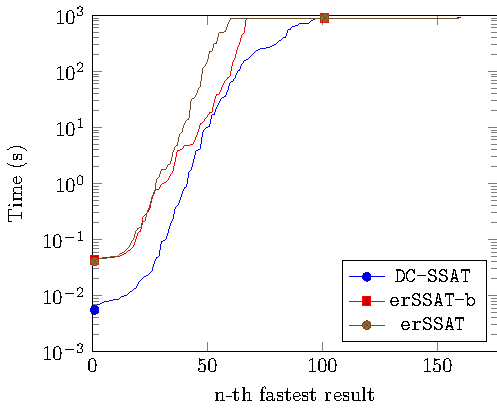
\includegraphics{exist-random-ssat/evaluation/plots/quantile-cputime-Application.pdf}
        \label{fig:erssat-quantile-cputime-application}
    }\\
    \subfloat[Memory usage]{
        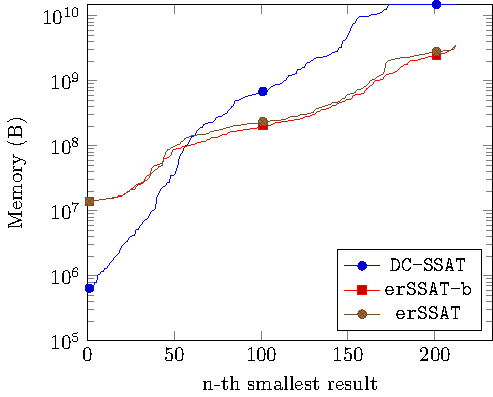
\includegraphics{exist-random-ssat/evaluation/plots/quantile-memory-Application.pdf}
        \label{fig:erssat-quantile-memory-application}
    }
    \caption{Quantile plots of application formulas}
    \label{fig:erssat-quantile-application}
\end{figure*}

\Cref{fig:erssat-quantile-application} shows the quantile plots of the application SSAT formulas.
We can see that the enhancement techniques affected not only the effectiveness of \erssat but also its efficiency
from~\cref{fig:erssat-quantile-cputime-application}.
This phenomenon indicates that the additional effort spent to strengthen a learnt clause is not worthy.
The reason behind this phenomenon will be inspected in the following.

\begin{figure*}[hp]
    \centering
    \subfloat[\erssatb]{
        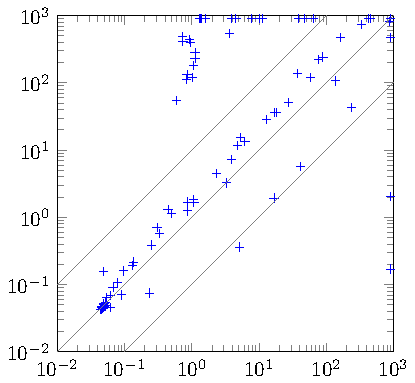
\includegraphics{exist-random-ssat/evaluation/plots/scatter-erssat.pdf}
        \label{fig:erssat-scatter-cputime-application}
    }\\
    \subfloat[\dcssat]{
        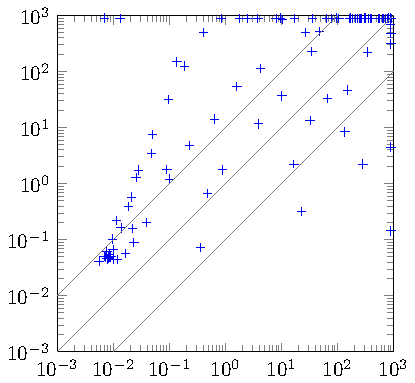
\includegraphics{exist-random-ssat/evaluation/plots/scatter-dcssat.pdf}
        \label{fig:dcssat-scatter-cputime-application}
    }
    \caption{CPU-time scatter plots of application formulas with \erssat in y-axis and compared approaches in x-axis}
    \label{fig:erssat-scatter-application}
\end{figure*}

To further examine the suitability of the enhancement techniques,
we demonstrate the scatter plots with \erssat in y-axis and compared approaches in x-axis
in~\cref{fig:erssat-scatter-application}.
A data point $(x,y)$ in the plots indicates that there is a formula processed by both \erssat and a compared approach,
while \erssat took a CPU time of $y$~seconds and the other approach took a CPU time of $x$~seconds.
From~\cref{fig:erssat-scatter-cputime-application},
we find that the enhancement techniques did improve the solving of some formulas,
but more often they were an overhead to \erssatb.
\Cref{fig:dcssat-scatter-cputime-application} also shows that
\dcssat was more efficient to exactly solve formulas than \erssat over the evaluated application formulas.

\subsubsection{Approximate solving}

\begin{table}[ht]
    \centering
    \scriptsize
    \caption{Results of solving the formulas from \textit{Conformant}}
    \label{tbl:exist-random-ssat-conformant}
    \begin{adjustbox}{angle=90}
        \pgfplotstabletypeset[
            every head row/.style={before row={\toprule
                            & \multicolumn{4}{c}{\dcssat} & \multicolumn{8}{c}{\erssat} & \multicolumn{8}{c}{\erssatb}\\},after row=\midrule},
            every last row/.style={after row=\bottomrule},
            empty cells with={--},
            formula column/.list={0},
            time column/.list={1,3,7},
            prob column/.list={2,4,8},
            lbound column/.list={5,9},
            lbtime column/.list={6,10}
        ]
        {exist-random-ssat/evaluation/csv/parsed-conformant.csv}
    \end{adjustbox}
\end{table}

\begin{table}[ht]
    \centering
    \scriptsize
    \caption{Results of solving the formulas from \textit{Max-Count}}
    \label{tbl:exist-random-ssat-maxcount}
    \begin{adjustbox}{angle=90}
        \pgfplotstabletypeset[
            every head row/.style={before row={\toprule
                            & \multicolumn{4}{c}{\dcssat} & \multicolumn{8}{c}{\erssat} & \multicolumn{8}{c}{\erssatb}\\},after row=\midrule},
            every last row/.style={after row=\bottomrule},
            empty cells with={--},
            formula column/.list={0},
            time column/.list={1,3,7},
            prob column/.list={2,4,8},
            lbound column/.list={5,9},
            lbtime column/.list={6,10}
        ]
        {exist-random-ssat/evaluation/csv/parsed-MaxCount.csv}
    \end{adjustbox}
\end{table}

\begin{table}[ht]
    \centering
    \scriptsize
    \caption{Results of solving the formulas from \textit{MPEC}}
    \label{tbl:exist-random-ssat-mpec}
    \begin{adjustbox}{angle=90}
        \pgfplotstabletypeset[
            every head row/.style={before row={\toprule
                            & \multicolumn{4}{c}{\dcssat} & \multicolumn{8}{c}{\erssat} & \multicolumn{8}{c}{\erssatb}\\},after row=\midrule},
            every last row/.style={after row=\bottomrule},
            empty cells with={--},
            formula column/.list={0},
            time column/.list={1,3,7},
            prob column/.list={2,4,8},
            lbound column/.list={5,9},
            lbtime column/.list={6,10}
        ]
        {exist-random-ssat/evaluation/csv/parsed-MPEC.csv}
    \end{adjustbox}
\end{table}

Recall that the proposed~\cref{alg:erssat} solves an SSAT formula in a converging manner.
Instead of computing the exact satisfying probability at once,
it keeps deriving lower bounds of the satisfying probability of a formula.
This characteristic integrates exact and approximate solving into one approach.
In the following, we study the approximation ability of \erssat.
We choose families \textit{Conformant}, \textit{Max-Count}, and \textit{MPEC} for detailed investigation,
because all of the compared approaches ran out of CPU time or memory over most of their formulas.

\Cref{tbl:exist-random-ssat-conformant,tbl:exist-random-ssat-maxcount,tbl:exist-random-ssat-mpec}
show the approximation results over the above three families, respectively.
For \dcssat, the CPU time and exact satisfying probability are reported.
For \erssat and \erssatb, in addition to the CPU and exact satisfying probability,
the tightest lower bound and the time elapsed to derive the lower bound are also shown in the tables.
A formula is not shown in the tables
if none of the approaches can solve it or derive a non-trivial lower bound for it.

As can be observed from the tables,
\erssat was able to derive tight lower bounds for formulas from these families,
while \dcssat suffered from timeouts over most of them.
The approximation ability of \erssat makes it useful for large formulas,
which cannot be exactly solved by the state-of-the-art approaches.

The above results on the random and application formulas suggest that:
\begin{itemize}
    \item The proposed solver \erssat achieves a similar performance as \dcssat in terms of CPU time and outperforms \dcssat in terms of memory consumption on random formulas.
    \item The proposed solver \erssat is not as good as \dcssat at exactly solving the application formulas, which can be attributed to the overhead caused by the enhancement techniques.
    \item The proposed solver \erssat is good at deriving tight lower bounds for large formulas. This approximation ability is especially valuable when the size of a formula is beyond the capability of the state-of-the-art exact solver.
\end{itemize}
To sum up, our evaluation results demonstrate the unique value of the proposed clause-containment learning.